\section{Auswertung}
\label{sec:Auswertung}

\subsection{Messung bis 1 bar}

Um die gemittelte Verdampfungswärme $L$ zu bestimmen, wird zunächst der
Logartithmus des Dampfdrucks gegen die reziproke absolute Temperatur
dargestellt und dann die gesuchte Größe mittels einer Ausgleichsrechnung
bestimmt.
\\
Die verwendeten Messwerte lassen sich in \autoref{tab:bis1} finden.
\\
\begin{table}
  \centering
  \caption{Messwerte bis 1 \si{\bar}}
  \label{tab:bis1}
  \sisetup{table-format=2.1}
  \begin{tabular}{cccc}
  \toprule
  $T_{Dampf} \,/\, \si{\celsius}$ & $T_{Dampf} \,/\, \si{\kelvin}$ & $p \,/\, \si{\milli\bar}$ & $p \,/\, \si{\pascal}$ \\
  \midrule
  17  & 290,15 & 35 & 77   \\
  19  & 292,15 & 45 & 67   \\
  20  & 293,15 & 55 &      \\
  21  & 294,15 & 61 &      \\
  22  & 295,15 & 65 &      \\
  23  & 296,15 & 68 &      \\
  24  & 297,15 & 74 &      \\
  25  & 298,15 & 78 &      \\
  26  & 299,15 & 81 &      \\
  27  & 300,15 & 85 &      \\
  28  & 301,15 & 90 &      \\
  29  & 302,15 & 95 &      \\
  30  & 303,15 & 99 &      \\
  31  & 304,15 & 104 &      \\
  32  & 305,15 & 107 &      \\
  33  & 306,15 & 111 &      \\
  34  & 307,15 & 118 &      \\
  35  & 308,15 & 122 &      \\
  36  & 309,15 & 127 &      \\
  37  & 310,15 & 133 &      \\
  38  & 311,15 & 137 &      \\
  39  & 312,15 & 144 &      \\
  40  & 313,15 & 150 &      \\
  41  & 314,15 & 153 &      \\
  42  & 315,15 & 160 &      \\
  43  & 316,15 & 166 &      \\
  44  & 317,15 & 175 &      \\
  45  & 318,15 & 184 &      \\
  46  & 319,15 & 190 &      \\
  47  & 320,15 & 194 &      \\
  48  & 321,15 & 199 &      \\
  49  & 322,15 & 208 &      \\
  50  & 323,15 & 217 &      \\
  51  & 324,15 & 226 &      \\
  52  & 325,15 & 232 &      \\
  53  & 326,15 & 240 &      \\
  54  & 327,15 & 252 &      \\
  55  & 328,15 & 260 &      \\
  56  & 329,15 & 269 &      \\
  57  & 330,15 & 278 &      \\
  58  & 331,15 & 290 &      \\
  59  & 332,15 & 305 &      \\
  60  & 333,15 & 324 &      \\
  61  & 334,15 & 339 &      \\
  62  & 335,15 & 360 &      \\
  63  & 336,15 & 378 &      \\
  64  & 337,15 & 399 &      \\
  65  & 338,15 & 437 &      \\
  66  & 339,15 & 450 &      \\
  67  &    & 463 &      \\
  68  &    & 481 &      \\
  69  &    & 485 &      \\
  70  &    & 496 &      \\
  71  &    & 521 &      \\
  72  &    & 528 &      \\
  73  &    & 542 &      \\
  74  &    & 551 &      \\
  75  &    & 569 &      \\
  76  &    & 582 &      \\
  77  &    & 603 &      \\
  78  &    & 617 &      \\
  79  &    & 640 &      \\
  80  &    & 647 &      \\
  81  &    & 663 &      \\
  82  &    & 678 &      \\
  83  &    & 688 &      \\
  84  &    & 711 &      \\
  85  &    & 722 &      \\
  86  &    & 730 &      \\
  87  &    & 736 &      \\
  88  &    & 753 &      \\
  89  &    & 765 &      \\
  90  &    & 770 &      \\
  91  &    & 778 &      \\
  92  &    & 790 &      \\
  93  &    & 793 &      \\
  94  &    & 811 &      \\
  95  &    & 816 &      \\
  96  &    & 825 &      \\
  97  &    & 830 &      \\
  98  &    & 836 &      \\
  99  &    & 837 &      \\
  \end{tabular} 
\end{table}

%\begin{figure}
%  \centering
%  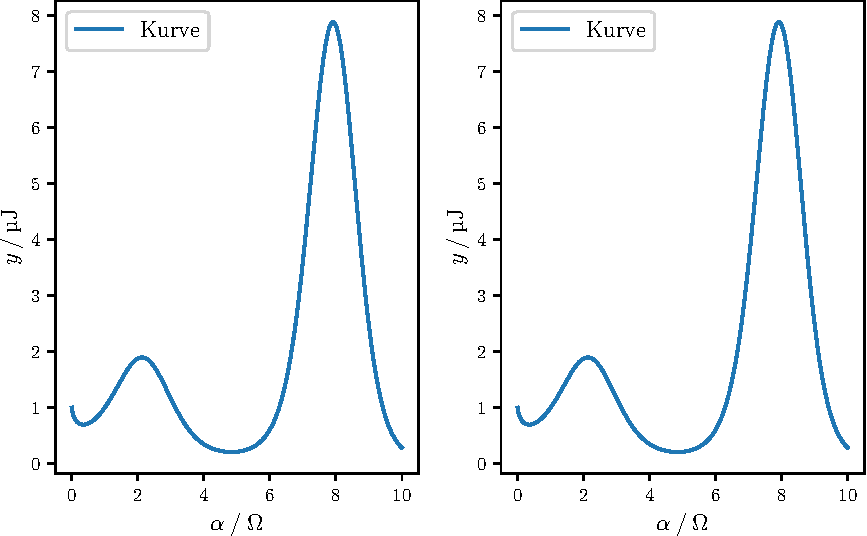
\includegraphics{plot.pdf}
%  \caption{Plot.}
%  \label{fig:plot}
%\end{figure}

